\chapter{Definición del Problema y Análisis}

\section{Formulación del Problema}

Actualmente la empresa Azalee cuenta con un prototipo para la medición de la porosidad y espesor oseo, este prototipo usa la técnica de transmisión axial para realizar las mediciones. Esta 
La transmisión axial es una técnica específicamente desarrollada para medir la propagación de ondas guiadas de ultrasonido en la capa cortical a lo largo del eje de los huesos. Los modos guiados propagados en la corteza son grabados con un arreglo de transductor lineal de 1-MHz. La medida de la curva de dispersión es obtenida usando una transformada de fourier de dos dimensiones (espacio, tiempo) combinada con una descomposición de valores singulares. La implementación actual de la interfaz humano-computador del prototipo tiene tiempos de respuesta mayor al deseado.

\section{Solución Propuesta}

La solución propuesta al problema consiste en revisar las etapas del algoritmo, modificar el código para reducir complejidades temporales. Analizar el rendimiento del software implementado para detectar los puntos problemáticos y las áreas dónde sea posible llevar a cabo una optimización del rendimiento.

\section{Objetivos}
A continuación se detallan los objetivos generales y específicos del trabajo de título
\begin{itemize}
    \item Qué: Qué realizaré. 
    \item Cómo: Cómo espero realizarlo (ej: tecnología). 
    \item Para qué: Por qué es necesario realizarlo. 
\end{itemize}

Además, los objetivos específicos deben ser consistentes con el objetivo general, y asegurar el alcanzarlo.

\subsection{Objetivo General}
\label{sc:OG}
Disminuir el tiempo de respuesta de la interfaz humano-computador del prototipo de mediciones corticales de huesos, optimizando las etapas del algoritmo.


\subsection{Objetivos Específicos}
\label{ssc:OE}
\begin{enumerate}
	\item Reducir complejidades temporales del algoritmo de análisis de datos.
	\item Analizar el rendimiento del software implementado (profiling). 
	\item Paralelizar código a nivel de datos y tareas.
	\item Acelerar el acceso a memoria ordenando los datos para tomar ventaja del cache del CPU.   
\end{enumerate}





\section{Metodología}
\label{sc:Met}

Se debe evidenciar coherencia entre la opción metodológica, el problema y los objetivos planteados.
Por otra parte, la realización de un esquema facilita la comprensión de su opción metodológica. Para finalizar, considere los tiempos de seminario de título al momento de definir una metodología.


En la Figura \ref{fig:met}, se presenta cómo insertar una imagen en \LaTeX{}.
\begin{figure}[H]
    \centering
    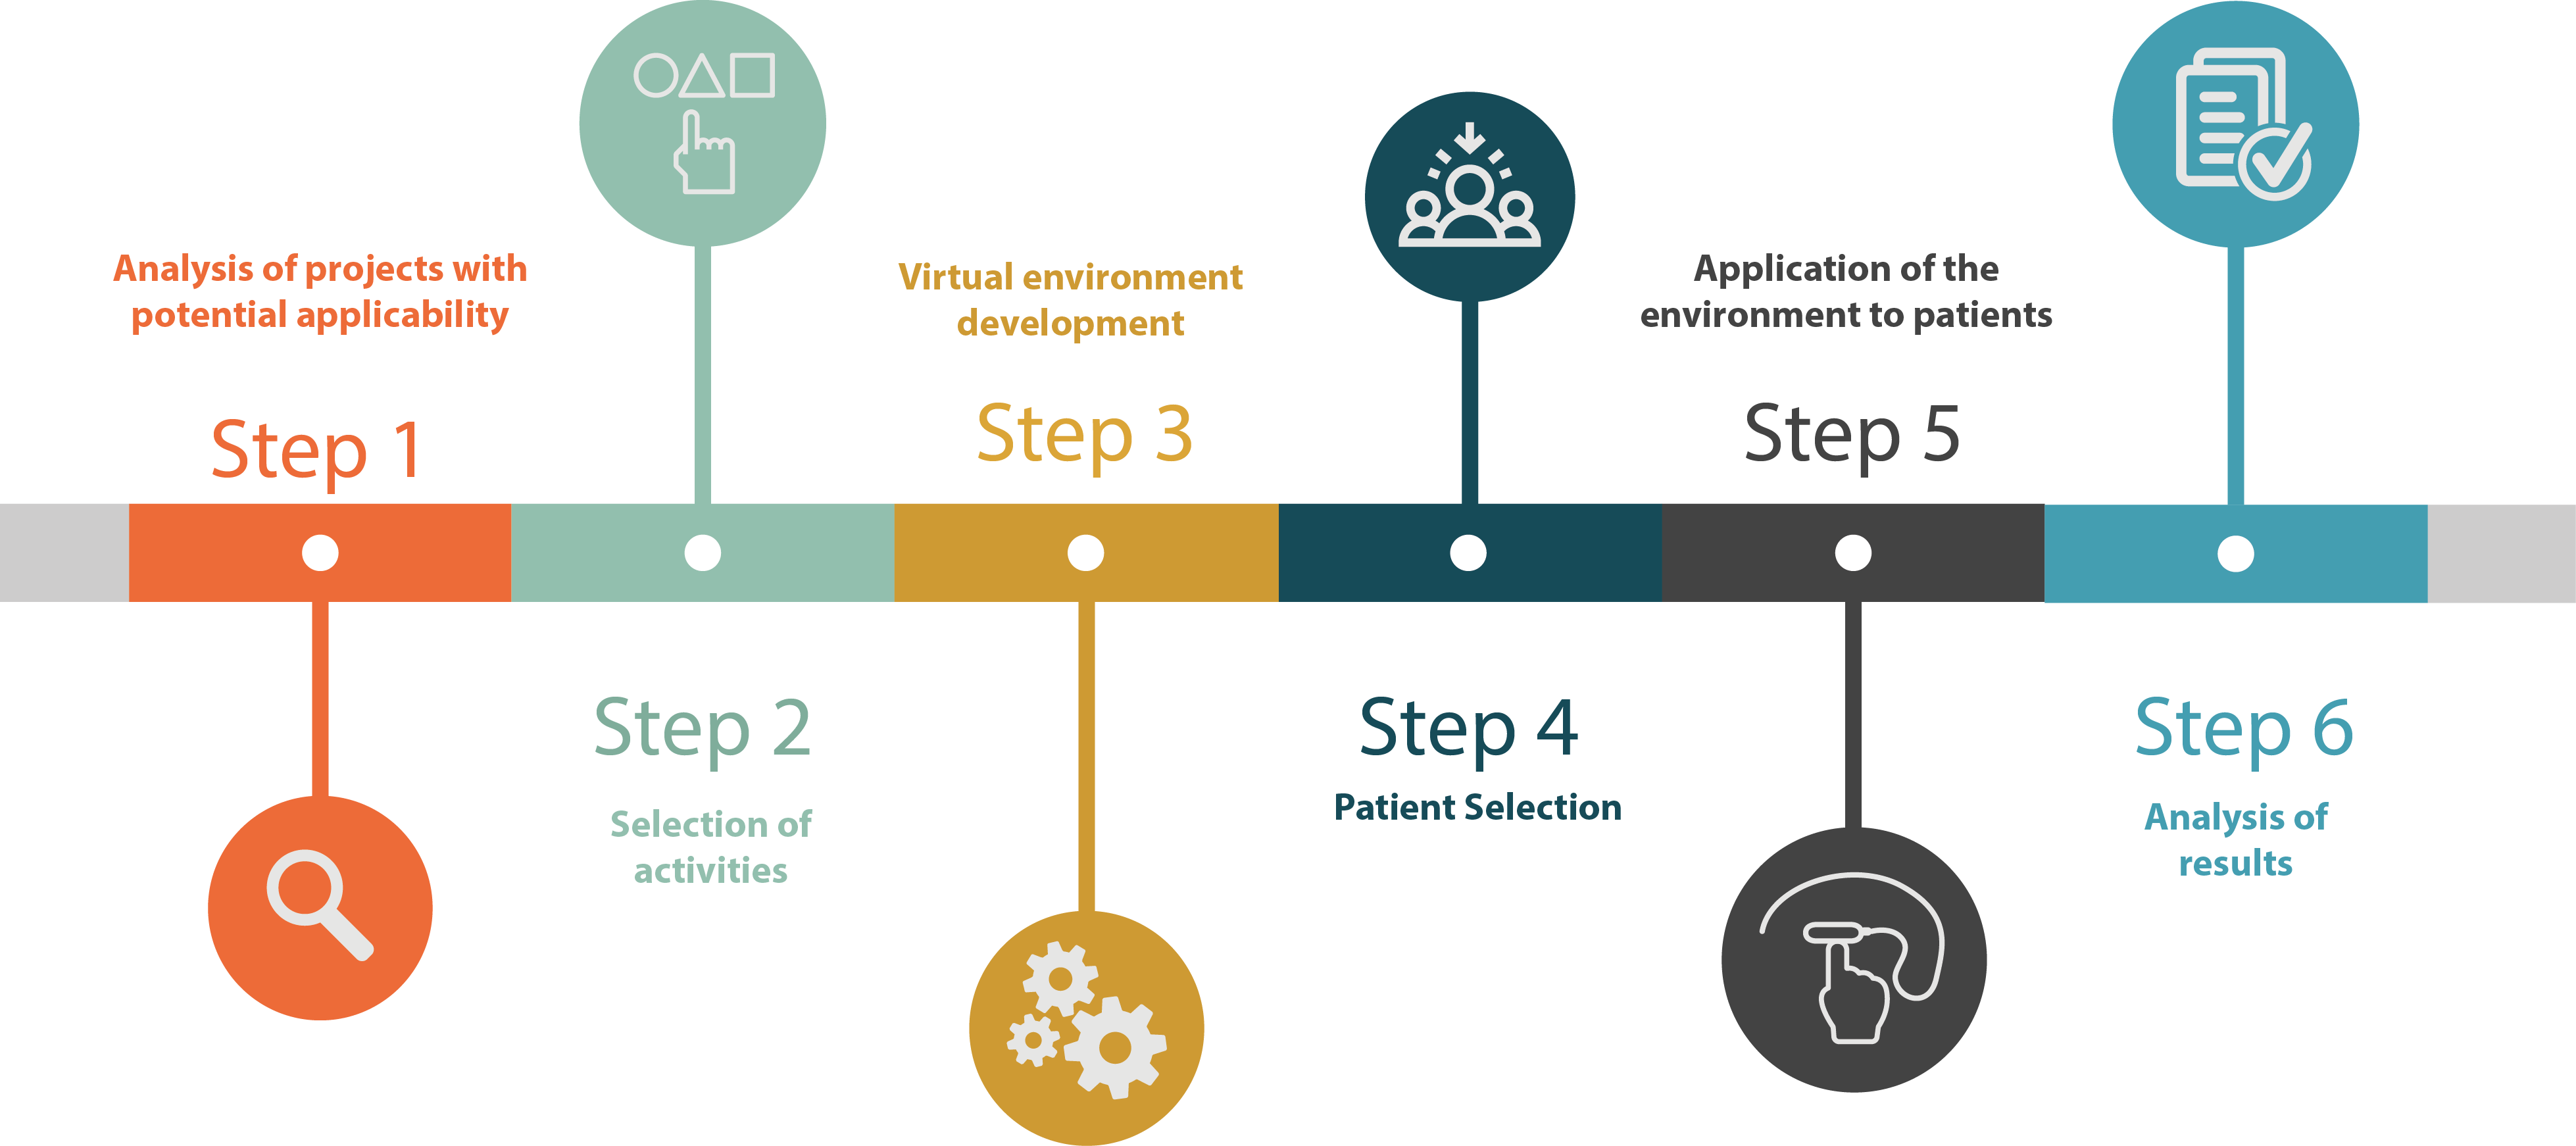
\includegraphics[width=0.75\textwidth]{imagenes/Fig_ejMet.png}
    \caption{Ejemplo de como insertar una figura}
    \label{fig:met}
\end{figure}



\section{Especificación de Requerimientos}
\label{sc:ER}


\subsection{Requerimientos Funcionales}
\label{ssc:RF}


\subsection{Requerimientos No Funcionales}
\label{ssc:RNF}
\section{Funcionalidades del Sistema}
\label{sc:FS}


\subsection{Diagramas de Casos de Uso}
\label{ssc:DCU}


\subsection{Casos de Uso}
\label{ssc:CU}

\subsection{Diagramas de Secuencia}
\label{ssc:DSS}

\subsection{Diagramas de Estado}
\label{ssc:DE}


\subsection{Modelo Conceptual}
\label{ssc:MC}